\documentclass[10pt]{article}\usepackage[]{graphicx}\usepackage[]{xcolor}
%% maxwidth is the original width if it is less than linewidth
%% otherwise use linewidth (to make sure the graphics do not exceed the margin)
\makeatletter
\def\maxwidth{ %
  \ifdim\Gin@nat@width>\linewidth
    \linewidth
  \else
    \Gin@nat@width
  \fi
}
\makeatother

\definecolor{fgcolor}{rgb}{0.345, 0.345, 0.345}
\newcommand{\hlnum}[1]{\textcolor[rgb]{0.686,0.059,0.569}{#1} }%
\newcommand{\hlstr}[1]{\textcolor[rgb]{0.192,0.494,0.8}{#1} }%
\newcommand{\hlcom}[1]{\textcolor[rgb]{0.678,0.584,0.686}{\textit{#1} } }%
\newcommand{\hlopt}[1]{\textcolor[rgb]{0,0,0}{#1} }%
\newcommand{\hlstd}[1]{\textcolor[rgb]{0.345,0.345,0.345}{#1} }%
\newcommand{\hlkwa}[1]{\textcolor[rgb]{0.161,0.373,0.58}{\textbf{#1} } }%
\newcommand{\hlkwb}[1]{\textcolor[rgb]{0.69,0.353,0.396}{#1} }%
\newcommand{\hlkwc}[1]{\textcolor[rgb]{0.333,0.667,0.333}{#1} }%
\newcommand{\hlkwd}[1]{\textcolor[rgb]{0.737,0.353,0.396}{\textbf{#1} } }%

\usepackage{framed}
\makeatletter
\newenvironment{kframe}{%
 \def\at@end@of@kframe{}%
 \ifinner\ifhmode%
  \def\at@end@of@kframe{\end{minipage} }%
  \begin{minipage}{\columnwidth}%
 \fi\fi%
 \def\FrameCommand##1{\hskip\@totalleftmargin \hskip-\fboxsep
 \colorbox{shadecolor}{##1}\hskip-\fboxsep
     % There is no \\@totalrightmargin, so:
     \hskip-\linewidth \hskip-\@totalleftmargin \hskip\columnwidth}%
 \MakeFramed {\advance\hsize-\width
   \@totalleftmargin\z@ \linewidth\hsize
   \@setminipage} }%
 {\par\unskip\endMakeFramed%
 \at@end@of@kframe}
\makeatother

\definecolor{shadecolor}{rgb}{.97, .97, .97}
\definecolor{messagecolor}{rgb}{0, 0, 0}
\definecolor{warningcolor}{rgb}{1, 0, 1}
\definecolor{errorcolor}{rgb}{1, 0, 0}
\newenvironment{knitrout}{}{} % an empty environment to be redefined in TeX

\usepackage{alltt}

%%%%%%%%%%%%%%%%%%%%%%%%%%%%%%%%%%%%%%%%%%%%%%%%%%%%%%%%%%%%%%%%%%%%%%%%%%%%%%%%
% LaTeX Imports
%%%%%%%%%%%%%%%%%%%%%%%%%%%%%%%%%%%%%%%%%%%%%%%%%%%%%%%%%%%%%%%%%%%%%%%%%%%%%%%%
\usepackage{amsfonts}                                                   % Math fonts
\usepackage{amsmath}                                                    % Math formatting
\usepackage{amssymb}                                                    % Math formatting
\usepackage{amsthm}                                                     % Math Theorems
\usepackage{arydshln}                                                   % Dashed hlines
\usepackage{attachfile}                                                 % AttachFiles
\usepackage{cancel}                                                     % Cancelled math
\usepackage{caption}                                                    % Figure captioning
\usepackage{color}                                                      % Nice Colors
\input{./lib/dragon.inp}                                                % Tikz dragon curve
\usepackage[ampersand]{easylist}                                        % Easy lists
\usepackage{fancyhdr}                                                   % Fancy Header
\usepackage[T1]{fontenc}                                                % Specific font-encoding
%\usepackage[margin=1in, marginparwidth=2cm, marginparsep=2cm]{geometry} % Margins
\usepackage{graphicx}                                                   % Include images
\usepackage{hyperref}                                                   % Referencing
\usepackage[none]{hyphenat}                                             % Don't allow hyphenation
\usepackage{lipsum}                                                     % Lorem Ipsum Dummy Text
\usepackage{listings}                                                   % Code display
\usepackage{marginnote}                                                 % Notes in the margin
\usepackage{microtype}                                                  % Niceness
\usepackage{lib/minted}                                                 % Code display
\usepackage{./lib/mlptikz}                                              % Tikz mlp
\usepackage{multirow}                                                   % Multirow tables
\usepackage{pdfpages}                                                   % Include pdfs
\usepackage{pgfplots}                                                   % Create Pictures
\usepackage{rotating}                                                   % Figure rotation
\usepackage{setspace}                                                   % Allow double spacing
\usepackage{subcaption}                                                 % Figure captioning
\usepackage{tikz}                                                       % Create Pictures
\usepackage{tocloft}                                                    % List of Equations
%%%%%%%%%%%%%%%%%%%%%%%%%%%%%%%%%%%%%%%%%%%%%%%%%%%%%%%%%%%%%%%%%%%%%%%%%%%%%%%%
% Package Setup
%%%%%%%%%%%%%%%%%%%%%%%%%%%%%%%%%%%%%%%%%%%%%%%%%%%%%%%%%%%%%%%%%%%%%%%%%%%%%%%%
\hypersetup{%                                                           % Setup linking
    colorlinks=true,
    linkcolor=black,
    citecolor=black,
    filecolor=black,
    urlcolor=black,
}
\RequirePackage[l2tabu, orthodox]{nag}                                  % Nag about bad syntax
\renewcommand*\thesection{\arabic{section} }                             % Reset numbering
\renewcommand{\theFancyVerbLine}{ {\arabic{FancyVerbLine} } }              % Needed for code display
\renewcommand{\footrulewidth}{0.4pt}                                    % Footer hline
\setcounter{secnumdepth}{3}                                             % Include subsubsections in numbering
\setcounter{tocdepth}{3}                                                % Include subsubsections in toc
%%%%%%%%%%%%%%%%%%%%%%%%%%%%%%%%%%%%%%%%%%%%%%%%%%%%%%%%%%%%%%%%%%%%%%%%%%%%%%%%
% Custom commands
%%%%%%%%%%%%%%%%%%%%%%%%%%%%%%%%%%%%%%%%%%%%%%%%%%%%%%%%%%%%%%%%%%%%%%%%%%%%%%%%
\newcommand{\nvec}[1]{\left\langle #1 \right\rangle}                    %  Easy to use vector
\newcommand{\inprod}[2]{\left\langle \vec{#1}, \vec{#2} \right\rangle}  %  Easy to use inner product
\newcommand{\norm}[1]{\lvert \lvert \vec{#1} \rvert \rvert}             %  Easy to use norm
\newcommand{\ma}[0]{\mathbf{A} }                                         %  Easy to use vector
\newcommand{\mb}[0]{\mathbf{B} }                                         %  Easy to use vector
\newcommand{\abs}[1]{\left\lvert #1 \right\rvert}                       %  Easy to use abs
\newcommand{\pren}[1]{\left( #1 \right)}                                %  Big parens
\let\oldvec\vec
\renewcommand{\vec}[1]{\mathbf{#1} }                            %  Vector Styling
\newtheorem{thm}{Theorem}                                               %  Define the theorem name
\theoremstyle{definition}
\newtheorem{definition}{Definition}                                     %  Define the definition name
\newtheorem{ex}{Example}                                                %  Define the example name
\definecolor{bg}{rgb}{0.95,0.95,0.95}
\newcommand{\java}[4]{\vspace{10pt}\inputminted[firstline=#2,
                                 lastline=#3,
                                 firstnumber=#2,
                                 gobble=#4,
                                 frame=single,
                                 label=#1,
                                 bgcolor=bg,
                                 linenos]{java}{#1} }
\newcommand{\python}[4]{\vspace{10pt}\inputminted[firstline=#2,
                                 lastline=#3,
                                 firstnumber=#2,
                                 gobble=#4,
                                 frame=single,
                                 label=#1,
                                 bgcolor=bg,
                                 linenos]{python}{#1} }
\newcommand{\js}[4]{\vspace{10pt}\inputminted[firstline=#2,
                                 lastline=#3,
                                 firstnumber=#2,
                                 gobble=#4,
                                 frame=single,
                                 label=#1,
                                 bgcolor=bg,
                                 linenos]{js}{#1} }
%%%%%%%%%%%%%%%%%%%%%%%%%%%%%%%%%%%%%%%%%%%%%%%%%%%%%%%%%%%%%%%%%%%%%%%%%%%%%%%%
% Beginning of document items - headers, title, toc, etc...
%%%%%%%%%%%%%%%%%%%%%%%%%%%%%%%%%%%%%%%%%%%%%%%%%%%%%%%%%%%%%%%%%%%%%%%%%%%%%%%%
\pagestyle{fancy}                                                       %  Establishes that the headers will be defined
\fancyhead[LE,LO]{Matrix Methods Notes}                                  %  Adds header to left
\fancyhead[RE,RO]{Zoe Farmer}                                       %  Adds header to right
\cfoot{\mlptikz[size=0.25in, text=on, textposx=0, textposy=0, textvalue=\thepage, textscale=0.75in]{applejack} }
\lfoot{APPM 3310}
\rfoot{Beylkin}
\title{Matrix Methods Notes}
\author{Zoe Farmer}

%%%%%%%%%%%%%%%%%%%%%%%%%%%%%%%%%%%%%%%%%%%%%%%%%%%%%%%%%%%%%%%%%%%%%%%%%%%%%%%%
% Beginning of document items - headers, title, toc, etc...
%%%%%%%%%%%%%%%%%%%%%%%%%%%%%%%%%%%%%%%%%%%%%%%%%%%%%%%%%%%%%%%%%%%%%%%%%%%%%%%%
\pagestyle{fancy}                                                 %  Establishes that the headers will be defined
\fancyhead[LE,LO]{Problem Set 8}                                  %  Adds header to left
\fancyhead[RE,RO]{Zoe Farmer, Jeremy Granger, Ryan Roden}     %  Adds header to right
\cfoot{\mlptikz[size=0.25in, text=on, textposx=0, textposy=0, textvalue=\thepage, textscale=0.75in]{applejack} }
\lfoot{CSCI 3104}
\rfoot{Clauset}
\title{Problem Set Eight}
\author{Zoe Farmer\\Jeremy Granger\\Ryan Roden}
%%%%%%%%%%%%%%%%%%%%%%%%%%%%%%%%%%%%%%%%%%%%%%%%%%%%%%%%%%%%%%%%%%%%%%%%%%%%%%%%
% Beginning of document items - headers, title, toc, etc...
%%%%%%%%%%%%%%%%%%%%%%%%%%%%%%%%%%%%%%%%%%%%%%%%%%%%%%%%%%%%%%%%%%%%%%%%%%%%%%%%
\IfFileExists{upquote.sty}{\usepackage{upquote} }{}
\begin{document}

\maketitle




\begin{easylist}[enumerate]
    @ First, review the material on depth-first spanning forests in Chapter 22.3 of the textbook. Then, consider the
    directed graph $G$ defined by the edge list

    \[
        G =
        \left\{
            (1, 2),
            (1, 4),
            (1, 8),
            (2, 3),
            (3, 1),
            (4, 8),
            (5, 2),
            (5, 6),
            (6, 2),
            (6, 3),
            (6, 5),
            (7, 4),
            (8, 7)
        \right\}
    \]

\begin{knitrout}
\definecolor{shadecolor}{rgb}{0.969, 0.969, 0.969}\color{fgcolor}\begin{figure}[H]


{\centering \includegraphics[width=\maxwidth]{figure/ps8_1network} 

}

\caption[Network]{Network\label{fig:ps8.1network} }
\end{figure}


\end{knitrout}


    @@ Draw the depth-first spanning forest, including and identifying all tree, back, forward, and cross edges. (If you
    prefer, you can identify the forward, back, and cross edges in separate lists instead of trying to draw and label
    them.)
    @@@ Please reference Table~\ref{table:edgetypes} for a list of edge types.

\begin{knitrout}
\definecolor{shadecolor}{rgb}{0.969, 0.969, 0.969}\color{fgcolor}\begin{figure}[H]


{\centering \includegraphics[width=\maxwidth]{figure/ps8_1forest} 

}

\caption[Depth-First Spanning Forest]{Depth-First Spanning Forest\label{fig:ps8.1forest} }
\end{figure}


\end{knitrout}


    \begin{table}[H]
        \centering
        \begin{tabular}{|l|l|l|}
            \hline
            1 & 2 & Forward\\
            1 & 4 & Cross\\
            1 & 8 & Forward\\
            2 & 3 & Forward\\
            3 & 1 & Back\\
            4 & 8 & Back\\
            5 & 2 & Back\\
            5 & 6 & Forward\\
            6 & 2 & Back\\
            6 & 3 & Back\\
            6 & 5 & Back\\
            7 & 4 & Forward\\
            8 & 7 & Forward\\
            \hline
        \end{tabular}
        \caption{Edge Types}
        \label{table:edgetypes}
    \end{table}

    @@ List all the strong components in $G$.
    @@@ A strong component is a strongly connected subgraph of $G$. There are three strong components in $G$:

    \[
        \left\{ (5,6), (1,2,3), (4,7,8) \right\}
    \]

    @ On an overnight camping trip at the Weathertop National Park you and your hobbit friend Samwise are woken from a
    restless sleep by a scream. Crawling out of your tent to investigate, you see a terrified park ranger running out of
    the woods, covered in blood and clutching a crumpled piece of paper to his chest. Reaching your tent, he gasps ``Get
    out\ldots while\ldots you\ldots'', thrusts the paper into your hands and falls to the ground, dead.

    Looking at the crumpled paper, you recognize a map of the park, drawn as an undirected graph, where vertices
    represent landmarks in the park, and edges represent trails between those landmarks. (Trails start and end at
    landmarks and do not cross.) Coincidentally, you recognize one of the vertices as your current location; several
    vertices on the boundary of the map are labeled EXIT.

    On closer examination, you notice that someone (perhaps the dead ranger) has written a real number between 0 and 1
    next to each vertex and each edge. A scrawled note on the back of the map indicates that a number next to a vertex
    or edge is the probability of encountering a deadly ringwraith along the corresponding trail or landmark. The note
    warns you that stepping off the marked trails will surely result in death.  You glance down at the corpse at your
    feet. His death certainly looked painful. On closer examination, you realize that the ranger is not dead at all, or
    rather, is turning into a wraith who will surely devour you. After burning the undead ranger's body, you wisely
    decide to leave the park immediately.
    @@ Give a (small) example $G$ such that the path from your current location to the EXIT node that minimizes the
    \textit{expected number} of encountered ringwraiths is different from the path that minimizes the
    \textit{probability of encountering any} ringwraiths at all. Explain why, in general, these two criteria lead to
    difference answers.
    @@@ If we let $X$ be the random variable indicating how ringwraiths are encountered, we can defined its expected
    value to be

    \[
        E(X) = \sum_{i = 0}^l x_i \cdot p(x_i)
    \]

    Where $x_i$ is the edge's index in the given path, and $p(x_i)$ is the probability of the corresponding edge. This
    probability distribution function is defined as

    \[
        f(X = k; l) =
        \begin{cases}
            p^k \cdot (1 - p)^{l - k} &\to k \in \left\{ 0, 1, \ldots, l \right\}\\
            0 &\to Otherwise
        \end{cases}
    \]

    Where $l$ is the length of the chosen path. Also known is the formula to determine the probability of encountering
    zero ringwraiths on the journey, which is defined as

    \[
        P(X=0) = \prod^l_{i=0} (1 - p_i)
    \]

    Where $l$ is again the length of the path and $p_i$ is the probability of encountering a ringwraith on that leg of
    the journey. We can now define a small network that demonstrates the requirement.

\begin{knitrout}
\definecolor{shadecolor}{rgb}{0.969, 0.969, 0.969}\color{fgcolor}\begin{figure}[H]


{\centering \includegraphics[width=\maxwidth]{figure/ps8_2a} 

}

\caption[Example $G$]{Example $G$\label{fig:ps8.2a} }
\end{figure}


\end{knitrout}


    We can now look at all paths and identify the minimums and maximums.

    \begin{table}[H]
        \centering
        \begin{tabular}{|l|l|l|}
            \hline
            Path & $P(X=0)$ & $E(X)$\\
            \hline
            {\ttfamily START -> 0.48 -> EXIT} &
                $0.0835$ &
                $1.5658$\\
            \hline
            {\ttfamily START -> 0.32 -> EXIT} &
                $0.0789$ &
                $1.508$\\
            \hline
            {\ttfamily START -> 0.48 -> 0.32 -> EXIT} &
                $0.0127$ &
                $2.5603$\\
            \hline
            {\ttfamily START -> 0.32 -> 0.48 -> EXIT} &
                $0.1226$ &
                $1.6792$\\
            \hline
        \end{tabular}
        \caption{Path Probabilities}
        \label{table:ring_probs}
    \end{table}

    In Table~\ref{table:ring_probs} we see that the optimal path for encountering no ringwraiths is {\ttfamily START ->
    0.32 -> 0.48 -> EXIT}, while the optimal path for encountering a minimal number of expected ringwraiths is {\ttfamily START
    -> 0.32 -> EXIT}.

    @@ Describe and analyze an efficient algorithm to find a path from your current location to an arbitrary EXIT node,
    such that the \textit{total expected number} of ringwraiths encountered along the path is as small as possible. Be
    sure to account for both the vertex probabilities and the edge probabilities.

    Gandalf's Hint: This is clearly and SSSP problem, but you must identify how to reduce the input $G$ to a form that
    can be solved by SSSP. Remember to include the cost of this transformation in your running-time analysis.
    @@@ First, let us define our network as a series of nodes in an adjacency matrix, where row or column indicates
    source or terminal node, and the value represents edge weight. We can now use Dijkstra's algorithm to determine
    SSSP. This algorithm examines our graph, starting with the source node, and looks at edge weights of all its
    adjacent edges. Let $V_i$ indicate our current vertex, with adjacent vertices $A_i$. For each adjacent vertex,
    examine the cost of traveling to that vertex through the current one (this cost is equal to the current node's cost,
    plus the cost of the edge between the current and adjacent vertices, plus the cost of the adjacent vertex) and if
    this new cost is less than the adjacent vertex's previous cost, update with the smaller. After all adjacent vertices
    have been examined, travel to the least costly adjacent vertex. Repeat until desired EXIT node is located.\newline

    Since this derivation of Dijkstra's original algorithm is almost identical, it also has $O(|V|)$ running time if we
    internally store vertices in a queue.

    @@ Describe and analyze an efficient algorithm to find a path from your current location to an arbitrary EXIT node,
    such that the \textit{probability of encountering any} ringwraiths at all is minimized.

    @@@ This is also a derivation of Dijkstra's algorithm, however our method of calculating the cost of a path has
    changed. For this algorithm, the cost of a path is now defined as the current node's cost, times the edge cost,
    times the next node's cost. We still select the lowest cost path after each analysis.\newline

    Again, since this derivation of Dijkstra's original algorithm is almost identical, it also has $O(|V|)$ running time
    if we internally store vertices in a queue.

    @ In a late night algorithms study session you and Golumn argue about the conditions under which a minimum spanning
    tree is unique. You agree that if all edges in $G$ have unique weights the MST is also unique, but you disagree
    about how to relax this assumption. Let $w(e)$ be a function that returns the weight of some $e \in E$.
    @@ Give an example of a (small) weighted graph that has both a unique MST and some $e$ and $e^\prime$ such that
    $w(e) = w(e^\prime) = x$.

    @@@ Demonstrated below.

\begin{knitrout}
\definecolor{shadecolor}{rgb}{0.969, 0.969, 0.969}\color{fgcolor}\begin{figure}[H]
\subfloat[Given Network\label{fig:ps8.3a1}]{

{\centering \includegraphics[width=0.45\textwidth]{figure/ps8_3a1} 

}

}
\subfloat[Unique MST\label{fig:ps8.3a2}]{

{\centering \includegraphics[width=0.45\textwidth]{figure/ps8_3a2} 

}

}\caption[Example $G$ and MST]{Example $G$ and MST\label{fig:ps8.3a} }
\end{figure}


\end{knitrout}


    If we use Kruskal's algorithm we can order all edges by their weights from smallest to largest. An edge is included
    as long as it does not make a cycle. If there are two minimum edge weights such that $w(e) = w(e^\prime)$, then we
    know that they will both be selected for our MST because the first two edges cannot make a cycle. Therefore since
    all other edges are distinct, you will end up with one minimum spanning tree. That is, whatever order of selecting
    the two minimum edges, the tree would be the same.

    @@ Golumn claims that the following is true. Prove via (small) counter examples that it is false.

    Golumn's Claim: $G$ has a unique MST if and only if (i) for any partition of the vertices of $G$ into two subsets
    the minimum-weight edge with one endpoint in each subset is unique and (ii) the maximum-weight edge in any cycle of
    $G$ is unique.
    @@@ If we partition our example graph (Figure~\ref{fig:3ba}) through edges $(V_4 , V_5)$ down to $(V_1, V_3)$ we see
    that, although the edge $(V_1, V_3)$ is the minimum weight edge with one endpoint in each subset, it is not unique
    ($(V_1 , V_3) = (V_1, V_2)$), yet the Minumum Spanning Tree for our graph is still unique.

    \begin{figure}[H]
        \centering
        \includegraphics[scale=0.5]{./img/ps8/3b1.png}
        \caption{$G$ Divided}
        \label{fig:3ba}
    \end{figure}

    We see that Figure~\ref{fig:3bb} still only has one unqiue Minumum Spanning Tree, yet the maximum weight edges
    $(V_4, V_5)$ and $(V_3, V_4)$ are \textit{not} unique. Thus, it is possible that a graph with non-unique minimum
    weight edges and/or non-unique maximum weight edges has a unique MST, and Gollumn is incorrect.

    \begin{figure}[H]
        \centering
        \includegraphics[scale=0.5]{./img/ps8/3b2.png}
        \caption{$G$'s MST}
        \label{fig:3bb}
    \end{figure}

    @@ Golumn now demands that you produce the correct relaxed condition, which you claim is the following. Prove that
    you are correct.

    Your Claim: An edge-weighted graph $G$ has a unique MST $T_{mst}$ if and only if the following conditions hold:
    (i) for any bipartation of the vertices induced by removing some edge $e \in T_{mst}$ the minimum-weight edge with
    one endpoint in each subset is unique, and
    (ii) the maximum-weight edge of any cycle constructed by adding on edge $f$ to $T_{mst}$, where $f \not\in T_{mst}$
    is unique.

    Gandalf's Hist: Note that for any spanning tree $T$ on $G$, removing some edge $e \in T$ induces a bipartation of
    the vertices. Consider the edges that span this cut.
    @@@ For this claim, we can prove using contradiction, making use of Professor Clauset's graph from his Lecture 23-25
    notes.

    \begin{figure}[H]
        \centering
        \includegraphics[scale=0.5]{./img/ps8/3ca.png}
        \caption{Clauset's Graph}
        \label{fig:3bb}
    \end{figure}

    Examining part i), if we suppose that we were to remove edge $(C, D)$, and that edges $(A, B)$ and $(G, F)$ have the
    same weight, $w=8$.

    \begin{figure}[H]
        \centering
        \includegraphics[scale=0.5]{./img/ps8/3cb.png}
        \caption{Adjusted Clauset's Graph}
        \label{fig:3bb}
    \end{figure}

    Since edges $(A, B)$ and $(F, G)$ are \textit{both} minimum weight edges, either edge could be used as the connector
    with one endpoint in each of our subtrees. The simple fact that we have a choice and that, in choosing one edge over
    the other, we have the same total weighted tree $w(G)$ either way, means that graph $G$ \textit{does not} have a
    unique minimum spanning tree, and that in order to have one, graph $G$ must have unique edges for any cut we decide
    to make.\newline

    For part ii) of our claim, suppose we have a graph with non-unique maximum edges with which to make a cycle.

    \begin{figure}[H]
        \centering
        \includegraphics[scale=0.5]{./img/ps8/3cc.png}
        \caption{Mondified Clauset's Graph for Part ii}
        \label{fig:3bb}
    \end{figure}

    Since edges $(A, B)$ and $(B, C)$ are maximums, both with the same weight $w=10$, the cycle induced by adding either
    of these edges to $G$'s MST would equate to the same weighted value of the MST. Therefore the MST would \textit{not}
    be unique. Any edges spanned by a cut in $G$ must be unique for the MST to be unique.

    @@ Describe and analyze an algorithm that will determine whether an input graph $G$ has a unique MST in
    (effectively) $O(E \lg V)$ time.

    Gandalf's Hint: Think about Kruskal's Algorithm.

    @@@ This algorithm is quite simple since our goal is only to find out if a given graph has a unique MST. We must
    create vertex sets using two vertices at a time. Then we need to compare each edge to see if it is a maximum weight,
    and if so, it is unique. Also, if it is not a maximum edge, we need to check to see if it is a minimum weight edge.
    If so, we need to check if it is unique. If in either condition we find two minimum or maximum edges that have the
    same weight, we know that our graph cannot possible have a unique MST and we're done. Following is the pseudo-code.

    \begin{pythoncode*}{gobble=8}
        def mst_unique(g):
            unique = True
            sort(Edge_Set_E).by_weight
            for vertix v in Vertices V:
                for each edge connected to vi:
                    compare safe_edges to current_edge:
                    if (v_is_min && w(v) &=& all w(vi) loop):
                        unique = False
                        break
                    elif (v_is_max && w(v) &=&  all w(vi) loop):
                        unique = False
                        break
            return unique
    \end{pythoncode*}

    Since this is a minor change from Kruskal's algorithm and navigates through all edges in the exact same way, the
    algorithm performs effectively in $O(E \log V)$ time. This is because we have only added a boolean value and
    comarison, which takes $O(1)$ time.

    @ Implement Dijkstra's algorithm for the SSSP problem using a binary min-heap, and show (in a nicely structed
    figure) that its running time is $O(E \lg V)$ on the following type of graphs.

    Recall from problem set 7 that $G(n, p)$ denotes a simple (undirected, unweighted, no self-loops) random graph with
    $n$ vertices in which each unordered pair $(u, v)$, where $u \neq v$, is connected with probability $p = c/(n - 1)$,
    for a constant expected degree $c$.  Let $G_d (n, p)$ denote a directed generalization of this model in which we
    relax the undirected requirement by letting each ordered pair $(u, v)$, where $u \neq v$, be connected with
    probability $p$. That is, instead of flipping $\binom{n}{2}$ coins for the upper triangle of the adjacency matrix,
    we flip $n^2 - n$ coins (because we still prohibit self loops) for the upper and lower triangles. Let $G_d (n, p)$
    with $c = 5$ define the input graph for Dijkstra's algorithm.

    @@ The output graph looks as such:

    \begin{figure}[H]
        \centering
        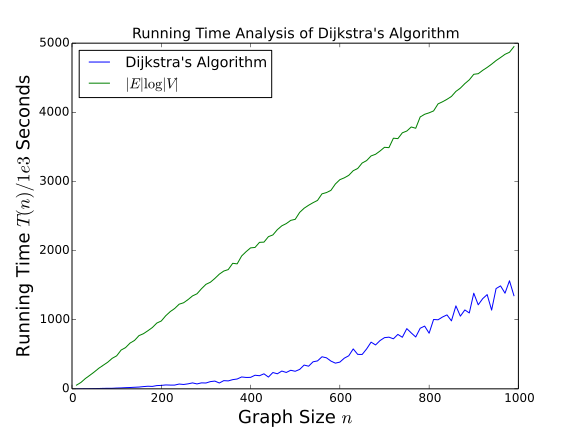
\includegraphics[scale=0.6]{./img/runtimeanalysis.png}
        \caption{Runtime Analysis}
    \end{figure}

    @ Currency arbitrage is a form of financial trading that uses discrepancies in foreign currency exchange rates to
    transform one unit of some currency into more than one unit of the same currency. For instance, suppose 1 U.S.\
    dollar bought 0.82 Euro, 1 Euro bought 129.7 Japanese Yen, 1 Japanese Yen bought 12 Turkish Lira and one Turkish
    Lira bought 0.0008 U.S.\ dollars. Then, by converting currencies, a trader could start with 1 U.S.\ dollar and buy
    $0.82 \times 129.7 \times 12 \times 0.0008 \approx 1.02 U.S.$ dollars, thus turning a 2\% profit. Of course, this is
    not how real currency markets work because each transaction must pay a commission to a middle-man for making the
    deal.

    Suppose that we are given $n$ currencies $c_1 , c_2 , \ldots , c_n$ and an $n \times n$ table $R$ of exchange rates,
    such that one unit of currency $c_i$ buys $R[i, j]$ units of currency $c_j$ . A traditional arbitrage opportunity is
    thus a cycle in the induced graph such that the product of the edge weights is greater than unity. That is, a
    sequence of currencies $\langle c_{i1} , c_{i 2} ,\ldots , c_{i k} \rangle$ such that $R[i_1 , i_2] \times R[i_2 ,
    i_3] \times \cdots \times R[i_{k-1} , i_k ] \times R[i_k , i_1 ] > 1$. Each transaction, however, must pay a
    commission, which is typically some $\alpha$ fraction of the transaction value, e.g., $\alpha = 0.01$ for a 1\%
    rate.

    @@ Give an efficient algorithm to determine whether or not there exists such an arbitrage
    opportunity, given a commission rate $\alpha$. Analyze the running time of your algorithm.

    Gandalf's hint: It is possible to solve this problem in $O(n^3)$. Recall that Bellman-Ford can be used to detect
    negative-weight cycles in a graph.
    @@@ The question asks to find a cycle such that

    \[
        R[1,2] \cdot R[2,3] \cdot \cdots \cdot R[k-1, k] \cdot R[k,1] > 1
    \]

    Inverting and taking the log of both sides gives us

    \[
        \log\left(\frac{1}{R[1,2]} \cdot \frac{1}{R[2,3]} \cdot \cdots
            \cdot \frac{1}{R[k-1, k]} \cdot \frac{1}{R[k,1]}\right) < \log(1) or 0
    \]

    Through logarithmic properties this is rewritten as

    \[
        \log\left(\frac{1}{R[1,2]}\right) +
            \log\left(\frac{1}{R[2,3]}\right) +
            \cdots + \log\left(\frac{1}{R[k-1,k]}\right) +
            \log\left(\frac{1}{R[k,1]}\right) < 0
    \]

    Changing the weights of each edge to the corresponding values above allows us to search for a negative cycle.

    Since we are looking for a negative cycle, we use the Bellman-Ford algorithm to accomplish this.  The problem asks
    for an efficient algorithm, and hints at Bellman-Ford which is $O(|V||E|) = O(|V|^3)$.  The nested for loops that
    change the currency conversions to the appropriate values for B-F runs in $O(|E|) = O(|V|^2)$, so this does not
    change the order of the runtime

    \begin{pythoncode*}{gobble=8}
        # Step 1: setup matrix to have proper values
        #         for Bellman-Ford and negative cycles
        matrix R = alpha*R

        for i from 1 to n {
          for j from 1 to n {
            R[i][j] = log(1/R[i][j]);
          }
        }

        BellmanFord( matrix R, vertex source, currencies n ){
          for v from 1 to n{
            if v is source, then distance[v] = 0;
            else distance[v] = infinity;
            p[v] = null;
          }

          //relax edges
          for v from 1 to n - 1{
            for i from 1 to n{
              for j from 1 to n{
                if distance[i] + R[i][j] < distance[j]
                  distance[j] = distance[i]+R[i][j]
                  p[j] = i;
              }
            }
          }

          //check for neg-weight cycles
          for i from 1 to n {
            for j from 1 to n {
              if distance[i] + R[i][j] < distance[j]
                FOUND NEGATIVE CYCLE
            }
          }
        }
    \end{pythoncode*}

    @@ Explain what effect varying $\alpha$ has on the structure of the set of possible arbitrage opportunities your
    algorithm might identify.
    @@@ Varying alpha will only change the amount of profit yielded from the arbitrage opportunity (as long as alpha is
    less than 100\%, in which case there would be no negative cycle ever), so it does not change the size of the set of
    arbitrage opportunities.
\end{easylist}

\end{document}
